
\documentclass{beamer}
\usecolortheme{dove}
\setbeamertemplate{navigation symbols}{}
\usepackage{amsmath,amssymb,amsfonts,amsthm, multicol, subfigure, color}
\usepackage{bm}
\usepackage{graphicx}
\usepackage{tabularx}
\usepackage{booktabs}
\usepackage{hyperref}
\usepackage{pdfpages}
\usepackage{xcolor}
\definecolor{seagreen}{RGB}{46, 139, 87}
\def\independenT#1#2{\mathrel{\rlap{$#1#2$}\mkern2mu{#1#2}}}
\newcommand\indep{\protect\mathpalette{\protect\independenT}{\perp}}
\def\log{\text{log}}
\newcommand\logit{\text{logit}}
\newcommand\iid{\stackrel{\text{iid}}{\sim}}
\newcommand\E{\text{E}}
\newcommand\V{\text{V}}
\renewcommand\P{\text{P}}
\newcommand{\Cov}{\text{Cov}}
\newcommand{\Cor}{\text{Cor}}
\newcommand\doop{\texttt{do}}
\usepackage{stackrel}
\usepackage{tikz}
\usetikzlibrary{arrows,shapes.arrows,positioning,shapes,patterns,calc}
\newcommand\slideref[1]{\vskip .1cm \tiny \textcolor{gray}{{#1}}}
\newcommand\red[1]{\color{red}#1}
\newcommand\blue[1]{\color{blue}#1}
\newcommand\gray[1]{\color{gray}#1}
\newcommand\seagreen[1]{\color{seagreen}#1}
\newcommand\purple[1]{\color{purple}#1}
\newcommand\orange[1]{\color{orange}#1}
\newcommand\black[1]{\color{black}#1}
\newcommand\white[1]{\color{white}#1}
\newcommand\teal[1]{\color{teal}#1}
\newcommand\magenta[1]{\color{magenta}#1}
\newcommand\Fuchsia[1]{\color{Fuchsia}#1}
\newcommand\BlueGreen[1]{\color{BlueGreen}#1}
\newcommand\bblue[1]{\textcolor{blue}{\textbf{#1}}}
\newcommand\bred[1]{\textcolor{red}{\textbf{#1}}}
\newcommand\bgray[1]{\textcolor{gray}{\textbf{#1}}}
\newcommand\bgreen[1]{\textcolor{seagreen}{\textbf{#1}}}
\newcommand\bref[2]{\href{#1}{\color{blue}{#2}}}
\colorlet{lightgray}{gray!40}
\pgfdeclarelayer{bg}    % declare background layer for tikz
\pgfsetlayers{bg,main} % order layers for tikz
\newcommand\mycite[1]{\begin{scriptsize}\textcolor{darkgray}{(#1)}\end{scriptsize}}
\newcommand{\tcframe}{\frame{
%\small{
\only<1|handout:0>{\tableofcontents}
\only<2|handout:1>{\tableofcontents[currentsubsection]}}
%}
}

\usepackage[round]{natbib}
\bibliographystyle{humannat-mod}
\setbeamertemplate{enumerate items}[default]
\usepackage{mathtools}

\newcommand{\goalsframe}{\begin{frame}{Learning goals for today}
At the end of class, you will be able to:
\begin{enumerate}
\item Apply matching estimators for causal effects
\item Use simulation to evaluate the bias, variance, and mean squared error of an estimator
\end{enumerate} \vskip .2in
\end{frame}}

\title{12. Matching Exercise}
\author{Ian Lundberg\\Cornell Info 6751: Causal Inference in Observational Settings\\Fall 2022}
\date{29 Sep 2022}

\begin{document}

\maketitle

\goalsframe

\begin{frame}{Simulation: Evaluating an estimator} \pause

Two broad classes of statistical research \pause
\begin{itemize}
\item Applications: Use an estimator to study the world \pause
\item Methodology: Study the performance of an estimator \pause
\end{itemize} \vskip .2in
To study methodology, it is often helpful to\\operate in a setting where the \bblue{truth is known}

\end{frame}

\begin{frame}{Simulate a population} \pause

Suppose we generate a population as follows.
\begin{center}
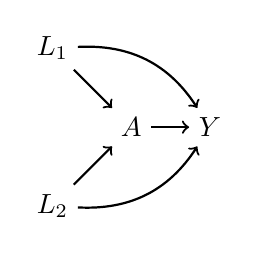
\begin{tikzpicture}
\node (l1) at (0,1) {$L_1$};
\node (l2) at (0,-1) {$L_2$};
\node (a) at (1,0) {$A$};
\node (y) at (2,0) {$Y$};
\draw[->, thick] (l1) to[bend left] (y);
\draw[->, thick] (l2) to[bend right] (y);
\draw[->, thick] (l1) -- (a);
\draw[->, thick] (l2) -- (a);
\draw[->, thick] (a) -- (y);
\end{tikzpicture}
\end{center} \pause
\begin{footnotesize}
$$\begin{aligned}
L_1 &\sim \text{Normal}(\text{Mean} = 0, \text{SD} = 1) \\ \pause
L_2 &\sim \text{Normal}(\text{Mean} = 0, \text{SD} = 1) \\ \pause
A &\sim \text{Bernoulli}\left(\text{logit}^{-1}\left[-2 + L1 + L2\right]\right) \\ \pause
Y^0 &\sim \text{Normal}\left(\text{Mean} = L1 + L2, SD = 1\right) \\ \pause
Y^1 &\sim \text{Normal}\left(\text{Mean} = L1 + L2 + 1, SD = 1\right) \\ \pause
Y &= \begin{cases} 
	Y^0 &\text{if }A=0 \\
	Y^1 &\text{if }A=1
	\end{cases}
\end{aligned}$$
\end{footnotesize} \pause
Generate a population of $N = 100,000$ cases

\end{frame}

\begin{frame}{Simulate samples}

\onslide<4->{For replication $1,\dots,R$,}
\begin{enumerate}
\item Sample $n = 100$ cases from the population \pause
\item Apply an estimator \pause
\item Produce a sample-based estimate $\hat\tau$
\end{enumerate}
\onslide<5->{Compare the distribution of our sample-based estimates to the known population truth $\tau$}

\end{frame}

\begin{frame}{Performance of the estimator: Visual summary}

\includegraphics[width = .8\textwidth]{figures/simulation_histogram}

\end{frame}

\begin{frame}{Performance of the estimator: Numeric summaries}

$$\begin{aligned}
&\text{Bias} && \frac{1}{R}\sum_{r=1}^R \left(\hat\tau_r - \tau\right) \\
&&&\text{Average error}\\ \\
&\text{Variance} && \frac{1}{R}\sum_{r=1}^R \left(\hat\tau_r - \bar{\hat\tau}\right)^2 \\
&&&\text{Sampling variation}\\ \\
&\text{Mean Squared Error} && \frac{1}{R}\sum_{r=1}^R \left(\hat\tau_r - \tau\right)^2 \\
&&&\text{How far off, on average}
\end{aligned}$$

\end{frame}

\begin{frame}{Exercise: Simulate performance of matching estimators}

In small groups, we will
\begin{itemize}
\item apply a matching estimator in a simulated setting
\item and assess its performance across repeated samples
\end{itemize} \vskip .2in
Exercise: \bref{https://tinyurl.com/MatchingSim}{tinyurl.com/MatchingSim}

\end{frame}

\goalsframe

\begin{frame}{Let me know what you are thinking}

\begin{huge} \bref{https://tinyurl.com/CausalQuestions}{tinyurl.com/CausalQuestions} \end{huge}
\vskip .7in

Office hours TTh 11am-12pm and at \bref{https://calendly.com/ianlundberg/office-hours}{calendly.com/ianlundberg/office-hours}\\Come say hi!

\end{frame}

\end{document}

